%%%----http://www.r-bloggers.com/imputing-missing-data-with-r-mice-package/

Imputing missing data with R; MICE package
October 4, 2015
By Michy Alice

(This article was first published on DataScience+, and kindly contributed to R-bloggers)

Missing data can be a not so trivial problem when analysing a dataset and accounting for it is usually not so straightforward either.

If the amount of missing data is very small relatively to the size of the dataset, then leaving out the few samples with missing features may be the best strategy in order not to bias the analysis, however leaving out available datapoints deprives the data of some amount of information and depending on the situation you face, you may want to look for other fixes before wiping out potentially useful datapoints from your dataset.

While some quick fixes such as mean-substitution may be fine in some cases, such simple approaches usually introduce bias into the data, for instance, applying mean substitution leaves the mean unchanged (which is desirable) but decreases variance, which may be undesirable.

The mice package in R, helps you imputing missing values with plausible data values. These plausible values are drawn from a distribution specifically designed for each missing datapoint.

In this post we are going to impute missing values using a the airquality dataset (available in R).
For the purpose of the article I am going to remove some datapoints from the dataset.

\begin{framed}
\begin{verbatim}

data <- airquality
data[4:10,3] <- rep(NA,7)
data[1:5,4] <- NA
\end{verbatim}
\end{framed}

As far as categorical variables are concerned, replacing categorical variables is usually not advisable. Some common practice include replacing missing categorical variables with the mode of the observed ones, however, it is questionable whether it is a good choice. Even though in this case no datapoints are missing from the categorical variables, we remove them from our dataset (we can add them back later if needed) and take a look at the data using summary().

data <- data[-c(5,6)]
summary(data)

     Ozone           Solar.R           Wind             Temp      
 Min.   :  1.00   Min.   :  7.0   Min.   : 1.700   Min.   :57.00  
 1st Qu.: 18.00   1st Qu.:115.8   1st Qu.: 7.400   1st Qu.:73.00  
 Median : 31.50   Median :205.0   Median : 9.700   Median :79.00  
 Mean   : 42.13   Mean   :185.9   Mean   : 9.806   Mean   :78.28  
 3rd Qu.: 63.25   3rd Qu.:258.8   3rd Qu.:11.500   3rd Qu.:85.00  
 Max.   :168.00   Max.   :334.0   Max.   :20.700   Max.   :97.00  
 NA's   :37       NA's   :7       NA's   :7        NA's   :5  
Apparently Ozone is the variable with the most missing datapoints. Below we are going to dig deeper into the missing data patterns.
\end{frame}
%============================================ %
\begin{frame}
Quick classification of missing data
There are two types of missing data:

MCAR: missing completely at random. This is the desirable scenario in case of missing data.
MNAR: missing not at random. Missing not at random data is a more serious issue and in this case it might be wise to check the data gathering process further and try to understand why the information is missing. For instance, if most of the people in a survey did not answer a certain question, why did they do that? Was the question unclear?

\end{frame}
%====================================== %
\begin{frame}[fragile]
\frametitle{The MICE package}
\Large
Assuming data is MCAR, too much missing data can be a problem too. Usually a safe maximum threshold is 5\% of the total for large datasets. If missing data for a certain feature or sample is more than 5\% then you probably should leave that feature or sample out. We therefore check for features (columns) and samples (rows) where more than 5\% of the data is missing using a simple function
\end{frame}
%====================================== %
\begin{frame}[fragile]
	\frametitle{The MICE package}
	\Large
pMiss <- function(x){sum(is.na(x))/length(x)*100}
apply(data,2,pMiss)
apply(data,1,pMiss)

    Ozone   Solar.R      Wind      Temp 
24.183007  4.575163  4.575163  3.267974 

  [1]  25  25  25  50 100  50  25  25  25  50  25   0   0   0   0   0   0   0   0   0   0
 [22]   0   0   0  25  25  50   0   0   0   0  25  25  25  25  25  25   0  25   0   0  25
 [43]  25   0  25  25   0   0   0   0   0  25  25  25  25  25  25  25  25  25  25   0   0
 [64]   0  25   0   0   0   0   0   0  25   0   0  25   0   0   0   0   0   0   0  25  25
 [85]   0   0   0   0   0   0   0   0   0   0   0  25  25  25   0   0   0  25  25   0   0
[106]   0  25   0   0   0   0   0   0   0  25   0   0   0  25   0   0   0   0   0   0   0
[127]   0   0   0   0   0   0   0   0   0   0   0   0   0   0   0   0   0   0   0   0   0
[148]   0   0  25   0   0   0
\end{frame}
%====================================== %
\begin{frame}[fragile]
	\frametitle{The MICE package}
	\Large
We see that Ozone is missing almost 25% of the datapoints, therefore we might consider either dropping it from the analysis or gather more measurements. The other variables are below the 5% threshold so we can keep them. As far as the samples are concerned, missing just one feature leads to a 25% missing data per sample. Samples that are missing 2 or more features (>50%), should be dropped if possible.
\end{frame}
%====================================== %
\begin{frame}[fragile]
	\frametitle{The MICE package}
	\Large
\subsection{Using mice for looking at missing data pattern}
The mice package provides a nice function md.pattern() to get a better understanding of the pattern of missing data

library(mice)
md.pattern(data)

    Temp Solar.R Wind Ozone   
104    1       1    1     1  0
 34    1       1    1     0  1
  4    1       0    1     1  1
  3    1       1    0     1  1
  3    0       1    1     1  1
  1    1       0    1     0  2
  1    1       1    0     0  2
  1    1       0    0     1  2
  1    0       1    0     1  2
  1    0       0    0     0  4
       5       7    7    37 56
The output tells us that 104 samples are complete, 34 samples miss only the Ozone measurement, 4 samples miss only the Solar.R value and so on.


\end{frame}
%======================================= %
\begin{frame}
A perhaps more helpful visual representation can be obtained using the VIM package as follows

library(VIM)
aggr_plot <- aggr(data, col=c('navyblue','red'), numbers=TRUE, sortVars=TRUE, labels=names(data), cex.axis=.7, gap=3, ylab=c("Histogram of missing data","Pattern"))
Rplot


\end{frame}
%====================================== %
\begin{frame}[fragile]
	\frametitle{The MICE package}
	\Large
The plot helps us understanding that almost 70% of the samples are not missing any information, 22% are missing the Ozone value, and the remaining ones show other missing patterns. Through this approach the situation looks a bit clearer in my opinion.

\end{frame}
%=================================================== %
\begin{frame}

Another (hopefully) helpful visual approach is a special box plot

marginplot(data)
Rplot02
\begin{figure}
\centering
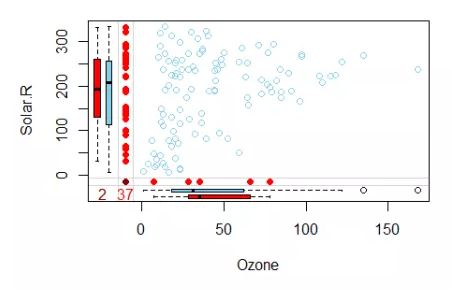
\includegraphics[width=0.7\linewidth]{Missing/MICE-02}
\caption{}
\label{fig:MICE-02}
\end{figure}


\end{frame}
%====================================== %
\begin{frame}[fragile]
	\frametitle{The MICE package}
	\Large
Obviously here we are constrained at plotting 2 variables at a time only, but nevertheless we can gather some interesting insights.
The red box plot on the left shows the distribution of Solar.R with Ozone missing while the blue box plot shows the distribution of the remaining datapoints. Likewhise for the Ozone box plots at the bottom of the graph.
If our assumption of MCAR data is correct, then we expect the red and blue box plots to be very similar.

\end{frame}
%======================================= %
\begin{frame}

Imputing the missing data
The mice() function takes care of the imputing process

tempData <- mice(data,m=5,maxit=50,meth='pmm',seed=500)
summary(tempData)

Multiply imputed data set
Call:
mice(data = data, m = 5, method = "pmm", maxit = 50, seed = 500)
Number of multiple imputations:  5
Missing cells per column:
  Ozone Solar.R    Wind    Temp 
     37       7       7       5 
Imputation methods:
  Ozone Solar.R    Wind    Temp 
  "pmm"   "pmm"   "pmm"   "pmm" 
VisitSequence:
  Ozone Solar.R    Wind    Temp 
      1       2       3       4 
PredictorMatrix:
        Ozone Solar.R Wind Temp
Ozone       0       1    1    1
Solar.R     1       0    1    1
Wind        1       1    0    1
Temp        1       1    1    0
Random generator seed value:  500 
\end{frame}
%========================================================== %
\begin{frame}[fragile]
A couple of notes on the parameters:

m=5 refers to the number of imputed datasets. Five is the default value.
meth='pmm' refers to the imputation method. In this case we are using predictive mean matching as imputation method. Other imputation methods can be used, type methods(mice) for a list of the available imputation methods.
If you would like to check the imputed data, for instance for the variable Ozone, you need to enter the following line of code

tempData$imp$Ozone

      1  2   3   4   5
5    13 20  28  12   9
10    7 16  28  14  20
25    8 14  14   1   8
26    9 19  32   8  37
...
The output shows the imputed data for each observation (first column left) within each imputed dataset (first row at the top).
\end{frame}
%=================================================== %
\begin{frame}[fragile]
If you need to check the imputation method used for each variable, mice makes it very easy to do

\begin{framed}
\begin{verbatim}
tempData$meth

Ozone Solar.R    Wind    Temp 
"pmm"   "pmm"   "pmm"   "pmm"
\end{verbatim}
\end{framed}

Now we can get back the completed dataset using the complete() function. It is almost plain English:

completedData <- complete(tempData,1)
The missing values have been replaced with the imputed values in the first of the five datasets. If you wish to use another one, just change the second parameter in the complete() function.
\end{frame}
%=================================================== %
\begin{frame}[fragile]
Inspecting the distribution of original and imputed data
Let’s compare the distributions of original and imputed data using a some useful plots.
First of all we can use a scatterplot and plot Ozone against all the other variables

xyplot(tempData,Ozone ~ Wind+Temp+Solar.R,pch=18,cex=1)
Here it is
Rplot03

\end{frame}
%=================================================== %
\begin{frame}
What we would like to see is that the shape of the magenta points (imputed) matches the shape of the blue ones (observed). The matching shape tells us that the imputed values are indeed “plausible values”.
Another helpful plot is the density plot:

densityplot(tempData)
Rplot04

\begin{figure}
\centering
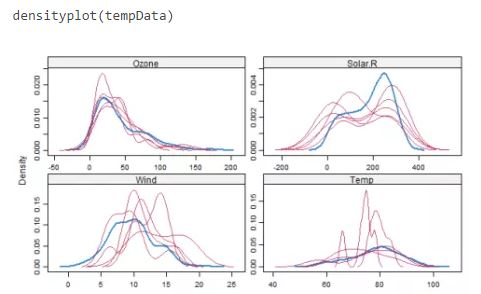
\includegraphics[width=0.7\linewidth]{Missing/MICE-04}
\caption{}
\label{fig:MICE-04}
\end{figure}

The density of the imputed data for each imputed dataset is showed in magenta while the density of the observed data is showed in blue. Again, under our previous assumptions we expect the distributions to be similar.
\end{frame}
%=================================================== %
\begin{frame}[fragile]
Another useful visual take on the distributions can be obtained using the stripplot() function that shows the distributions of the variables as individual points
%
%stripplot(tempData, pch = 20, cex = 1.2)
%Rplot05
\end{frame}
%=================================================== %
\begin{frame}

\begin{figure}
\centering
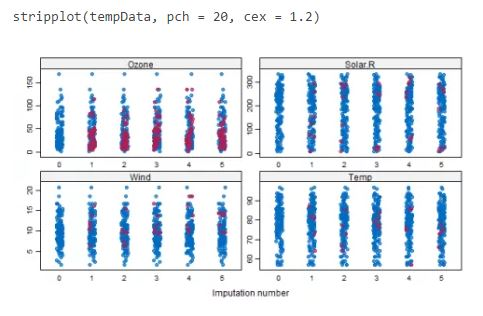
\includegraphics[width=0.7\linewidth]{Missing/MICE-05}
\end{figure}

\end{frame}
%========================================================== %
\begin{frame}
Pooling
Suppose that the next step in our analysis is to fit a linear model to the data. You may ask what imputed dataset to choose. The mice package makes it again very easy to fit a a model to each of the imputed dataset and then pool the results together
\end{frame}
%========================================================== %
\begin{frame}[fragile]

modelFit1 <- with(tempData,lm(Temp~ Ozone+Solar.R+Wind))
summary(pool(modelFit1))

                     est         se         t       df     Pr(>|t|)
(Intercept) 72.812078768 2.95380500 24.650266 84.18464 0.000000e+00
Ozone        0.163094287 0.02607674  6.254397 57.78569 5.236295e-08
Solar.R      0.009679676 0.00789576  1.225933 37.48960 2.278691e-01
Wind        -0.352582008 0.21639828 -1.629320 92.89136 1.066321e-01
                   lo 95       hi 95 nmis       fmi    lambda
(Intercept) 66.938301817 78.68585572   NA 0.1477818 0.1277731
Ozone        0.110891894  0.21529668   37 0.2155848 0.1888975
Solar.R     -0.006311604  0.02567095    7 0.3004189 0.2640672
Wind        -0.782312735  0.07714872    0 0.1300747 0.1115442

\end{frame}
%=================================================== %
\begin{frame}
The variable modelFit1 containts the results of the fitting performed over the imputed datasets, while the pool() function pools them all together. Apparently, only the Ozone variable is statistically significant.
Note that there are other columns aside from those typical of the lm() model: fmi contains the fraction of missing information while lambda is the proportion of total variance that is attributable to the missing data. For more information I suggest to check out the paper cited at the bottom of the page.
\end{frame}
%=================================================== %
\begin{frame}
Remember that we initialized the mice function with a specific seed, therefore the results are somewhat dependent on our initial choice. To reduce this effect, we can impute a higher number of dataset, by changing the default m=5 parameter in the mice() function as follows

tempData2 <- mice(data,m=50,seed=245435)
modelFit2 <- with(tempData2,lm(Temp~ Ozone+Solar.R+Wind))
summary(pool(modelFit2))
\end{frame}
%========================================================== %
\begin{frame}
                     est          se         t       df     Pr(>|t|)
(Intercept) 73.156084276 2.803010282 26.099114 129.3154 0.000000e+00
Ozone        0.166242781 0.024926976  6.669192 118.4408 8.645631e-10
Solar.R      0.009046835 0.007374103  1.226839 114.5471 2.223989e-01
Wind        -0.382700790 0.202976584 -1.885443 136.6735 6.149264e-02
                   lo 95       hi 95 nmis        fmi    lambda
(Intercept) 67.610387851 78.70178070   NA 0.11141367 0.0977762
Ozone        0.116882484  0.21560308   37 0.16290744 0.1488906
Solar.R     -0.005560458  0.02365413    7 0.18096774 0.1667911
Wind        -0.784081566  0.01867999    0 0.07425875 0.0608104
\end{frame}
%=================================================== %
\begin{frame}
After having taken into account the random seed initialization, we obtain (in this case) more or less the same results as before with only Ozone showing statistical significance.

A gist with the full code for this post can be found here.

Note: I learnt this technique in a paper entitled mice: Multivariate Imputation by Chained Equations in R by Stef van Buuren. It is a great paper and I highly recommend to read it if you are interested in multiple imputation!

Thank you for reading this post, leave a comment below if you have any question.
\end{frame}
%=================================================== %
\end{document}